
%(BEGIN_QUESTION)
% Copyright 2006, Tony R. Kuphaldt, released under the Creative Commons Attribution License (v 1.0)
% This means you may do almost anything with this work of mine, so long as you give me proper credit

Determine the correct potentiometer millivoltage setting to generate the following temperature indications on the following instruments:

$$\includegraphics[width=15.5cm]{i00422x01.eps}$$

\begin{itemize}
\item{} -100$^{o}$ F ; Potentiometer setting = ??? 
\item{} 150$^{o}$ F ; Potentiometer setting = ??? 
\item{} 400$^{o}$ F ; Potentiometer setting = ??? 
\end{itemize}

\vskip 10pt

$$\includegraphics[width=15.5cm]{i00422x02.eps}$$

\begin{itemize}
\item{} 0$^{o}$ F ; Potentiometer setting = ??? 
\item{} 375$^{o}$ F ; Potentiometer setting = ??? 
\item{} 750$^{o}$ F ; Potentiometer setting = ??? 
\end{itemize}

\vskip 10pt

$$\includegraphics[width=15.5cm]{i00422x03.eps}$$

\begin{itemize}
\item{} -50$^{o}$ F ; Potentiometer setting = ??? 
\item{} 975$^{o}$ F ; Potentiometer setting = ??? 
\item{} 2000$^{o}$ F ; Potentiometer setting = ??? 
\end{itemize}

\underbar{file i00422}
%(END_QUESTION)





%(BEGIN_ANSWER)

$$\includegraphics[width=15.5cm]{i00422x01.eps}$$

\begin{itemize}
\item{} -100$^{o}$ F ; Potentiometer setting = -4.598 mV (or, 4.598 mV connected in reverse polarity) 
\item{} 150$^{o}$ F ; Potentiometer setting = 2.307 mV 
\item{} 400$^{o}$ F ; Potentiometer setting = 9.920 mV 
\end{itemize}

\vskip 10pt

$$\includegraphics[width=15.5cm]{i00422x02.eps}$$

\begin{itemize}
\item{} 0$^{o}$ F ; Potentiometer setting = -1.452 mV (or, 1.452 mV connected in reverse polarity) 
\item{} 375$^{o}$ F ; Potentiometer setting = 12.298 mV 
\item{} 750$^{o}$ F ; Potentiometer setting = 28.431 mV 
\end{itemize}

\vskip 10pt

$$\includegraphics[width=15.5cm]{i00422x03.eps}$$

\begin{itemize}
\item{} -50$^{o}$ F ; Potentiometer setting = -3.364 mV (or 3.364 mV connected in reverse polarity) 
\item{} 975$^{o}$ F ; Potentiometer setting = 20.028 mV 
\item{} 2000$^{o}$ F ; Potentiometer setting = 43.231 mV 
\end{itemize}

%(END_ANSWER)





%(BEGIN_NOTES)


%INDEX% Measurement, temperature: thermocouple

%(END_NOTES)


